\documentclass{beamer}
\usetheme{Warsaw}
\usepackage{graphicx}
\usepackage{listings}
\usepackage{tikz}
\usepackage{tikz-qtree}
\lstset{language=tex,
basicstyle=\ttfamily\footnotesize,
frame=shadowbox,
breaklines=true}

\usepackage[utf8]{inputenc}

\DeclareMathOperator*{\argmax}{arg\,max}

\title{A Latex primer}

\author{Giuseppe Maggiore}

\institute{NHTV University of Applied Sciences \\
Breda, Netherlands}

\date

\begin{document}
\maketitle


\begin{frame}[fragile]{Empty document}
\begin{lstlisting}
\documentclass[10pt,a4paper]{book}
\usepackage[utf8]{inputenc}
\usepackage[english]{babel}
\usepackage{amsmath}
\usepackage{amsfonts}
\usepackage{amssymb}
\usepackage{graphicx}
\begin{document}
  ...
\end{document}
\end{lstlisting}
\end{frame}


\begin{frame}[fragile]{Title}
\begin{lstlisting}
\title{A presentation on Latex}
\author{Dr. Giuseppe Maggiore}
\maketitle
  ...
\end{lstlisting}
\end{frame}


\begin{frame}[fragile]{Sections and subsections}
\begin{lstlisting}
\section{Introduction}
  ...
  \subsection{Motivation}
    ...
  \subsection{Problem statement}
    ...
    \subsubsection{Points of interest of problem}
      ...
\end{lstlisting}
\end{frame}


\begin{frame}[fragile]{Text modifiers}
\begin{lstlisting}
Regular text, \textit{italic}, \textbf{bold}, 
  \texttt{typewriter}, \textsc{small caps}, 
  \textsf{sans serif}, \textsl{slanted}, 
  \emph{emphasis}
\end{lstlisting}
\begin{block}{Result}
Regular text, \textit{italic}, \textbf{bold}, \texttt{typewriter}, \textsc{small caps}, \textsf{sans serif}, \textsl{slanted}, \emph{emphasis}
\end{block}
\end{frame}


\begin{frame}[fragile]{Lists}
\begin{lstlisting}
\begin{itemize}
  \item First item
  \item Second item
    \begin{itemize}
      \item Nested list item 1
      \item Nested list item 2
    \end{itemize}
\end{itemize}
\end{lstlisting}
\begin{block}{Result}
\begin{itemize}
  \item First item
  \item Second item
    \begin{itemize}
      \item Nested list item 1
      \item Nested list item 2
    \end{itemize}
\end{itemize}
\end{block}
\end{frame}


\begin{frame}[fragile]{Lists}
\begin{lstlisting}
\begin{enumerate}
  \item First item
  \item Second item
    \begin{enumerate}
      \item Nested list item 1
      \item Nested list item 2
    \end{enumerate}
\end{enumerate}
\end{lstlisting}
\begin{block}{Result}
\begin{enumerate}
  \item First item
  \item Second item
    \begin{enumerate}
      \item Nested list item 1
      \item Nested list item 2
    \end{enumerate}
\end{enumerate}
\end{block}
\end{frame}


\begin{frame}[fragile]{Lists}
\begin{lstlisting}
\begin{description}
  \item[First] The first item
  \item[Second] The second item
  \item[Third] The third
\end{description}\end{lstlisting}
\begin{block}{Result}
\begin{description}
  \item[First] The first item
  \item[Second] The second item
  \item[Third] The third
\end{description}
\end{block}
\end{frame}


\begin{frame}[fragile]{Quotations}
\begin{lstlisting}
Isaac Newton summed up his own estimate of his work as follows:
\begin{quote}
I do not know what I may appear to the world; but to
myself I seem to have been only like a boy, playing
on the sea-shore, and diverting myself, in now and
then finding a smoother pebble, or a prettier shell
than ordinary, whilst the great ocean of truth lay
all undiscovered before me.
\end{quote}
\end{lstlisting}
\begin{block}{Result}
Isaac Newton summed up his own estimate of his work as follows:
\begin{quote}
I do not know what I may appear to the world; but to
myself I seem to have been only like a boy, playing
on the sea-shore, and diverting myself, in now and
then finding a smoother pebble, or a prettier shell
than ordinary, whilst the great ocean of truth lay
all undiscovered before me.
\end{quote}
\end{block}
\end{frame}


\begin{frame}[fragile]{Pre-formatted text}
\begin{lstlisting}
\verb/\alpha/
\end{lstlisting}
\begin{block}{Result}
\verb/\alpha/
\end{block}
\end{frame}


\begin{frame}[fragile]{Internal cross-references}
\begin{lstlisting}
\label{sec1:introduction}
As seen in \ref{sec1:introduction}, ...
\end{lstlisting}
\begin{block}{Result}
\label{sec1:introduction}
As seen in Section \ref{sec1:introduction}, ...
\end{block}
\end{frame}


\begin{frame}[fragile]{Tables}
\begin{lstlisting}
\begin{tabular}{|r|r|}
\hline
$n$&$n!$\\
\hline
1&1\\
2&2\\
3&6\\
\dots & \dots \\
\hline
\end{tabular}
\end{lstlisting}
\begin{block}{Result}
\begin{tabular}{|r|r|}
\hline
$n$&$n!$\\
\hline
1&1\\
2&2\\
3&6\\
\dots & \dots \\
\hline
\end{tabular}
\end{block}
\end{frame}


\begin{frame}[fragile]{Tables}
\fontsize{6}{7.2}\selectfont
\begin{lstlisting}
\begin{tabular}{|l||l|l||l|l|}
\hline
 &\multicolumn{2}{l|}{Singular}&\multicolumn{2}{l|}{Plural}\\
\cline{2-5}
 &English&\textbf{Gaeilge}&English&\textbf{Gaeilge}\\
\hline\hline
1st Person&at me&\textbf{agam}&at us&\textbf{againn}\\
2nd Person&at you&\textbf{agat}&at you&\textbf{agaibh}\\
\hline
\end{tabular}\end{lstlisting}
\begin{block}{Result}
\begin{tabular}{|l||l|l||l|l|}
\hline
 &\multicolumn{2}{l|}{Singular}&\multicolumn{2}{l|}{Plural}\\
\cline{2-5}
 &English&\textbf{Gaeilge}&English&\textbf{Gaeilge}\\
\hline\hline
1st Person&at me&\textbf{agam}&at us&\textbf{againn}\\
2nd Person&at you&\textbf{agat}&at you&\textbf{agaibh}\\
\hline
\end{tabular}
\end{block}
\end{frame}


\begin{frame}[fragile]{Figures}
\begin{lstlisting}
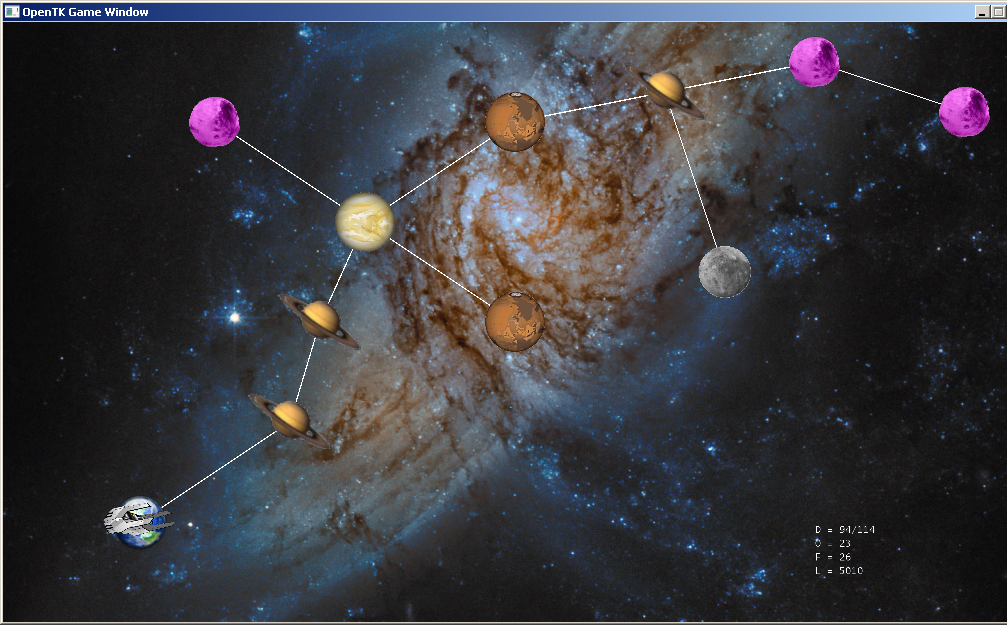
\includegraphics[width=4cm]{Pics/pic.png}
\end{lstlisting}
\begin{block}{Result}
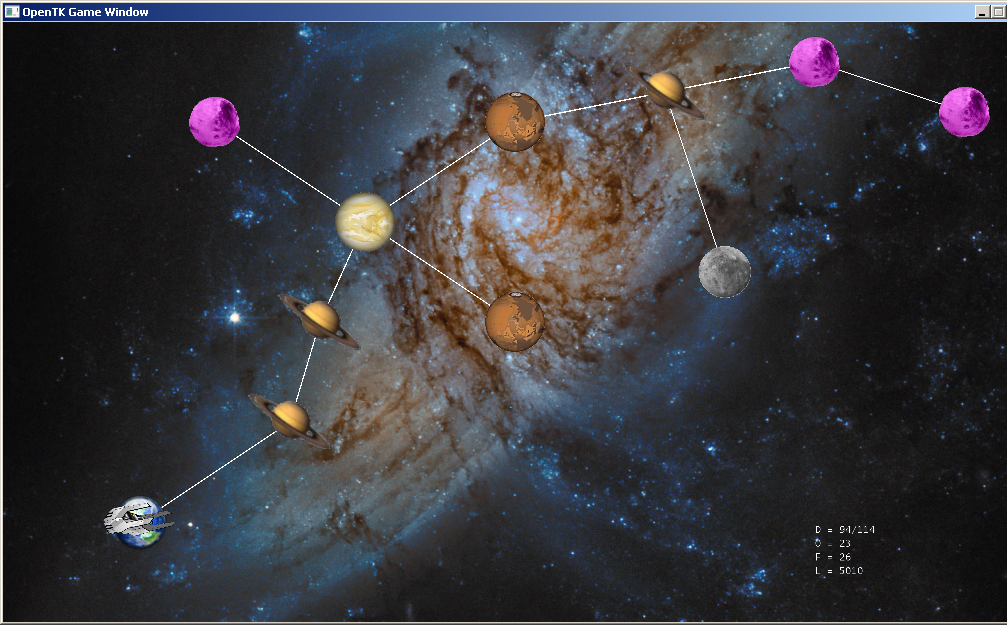
\includegraphics[width=4cm]{Pics/pic.png}
\end{block}
\end{frame}


\begin{frame}[fragile]{Figures}
\begin{lstlisting}
\begin{figure}
\centering
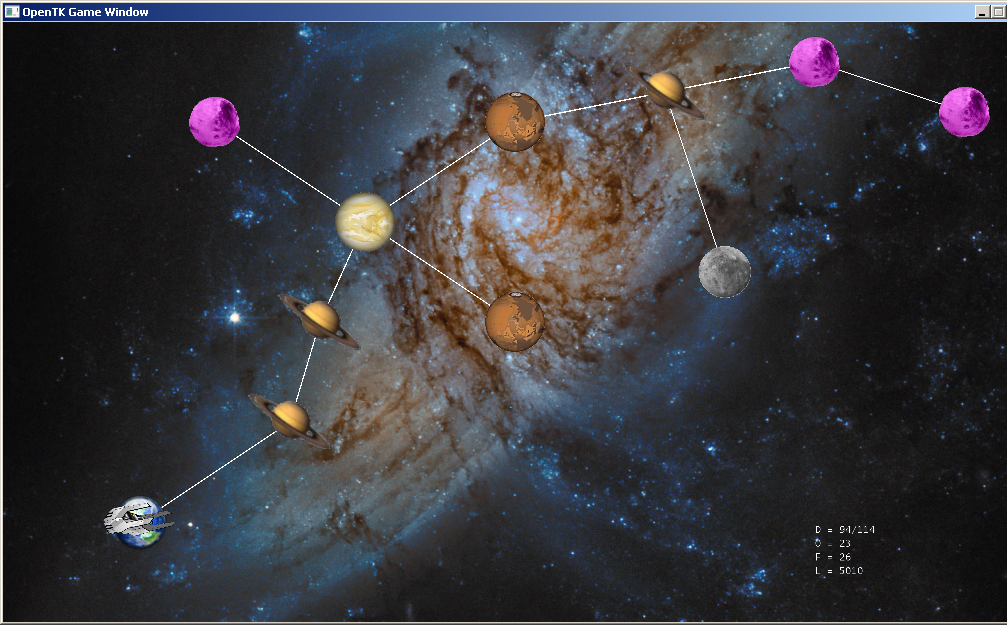
\includegraphics[width=4cm]{Pics/pic.png}
\caption{A planning AI simulator prototype}
\label{fig:AI-prototype}
\end{figure}
\end{lstlisting}
\begin{block}{Result}
\begin{figure}
\centering
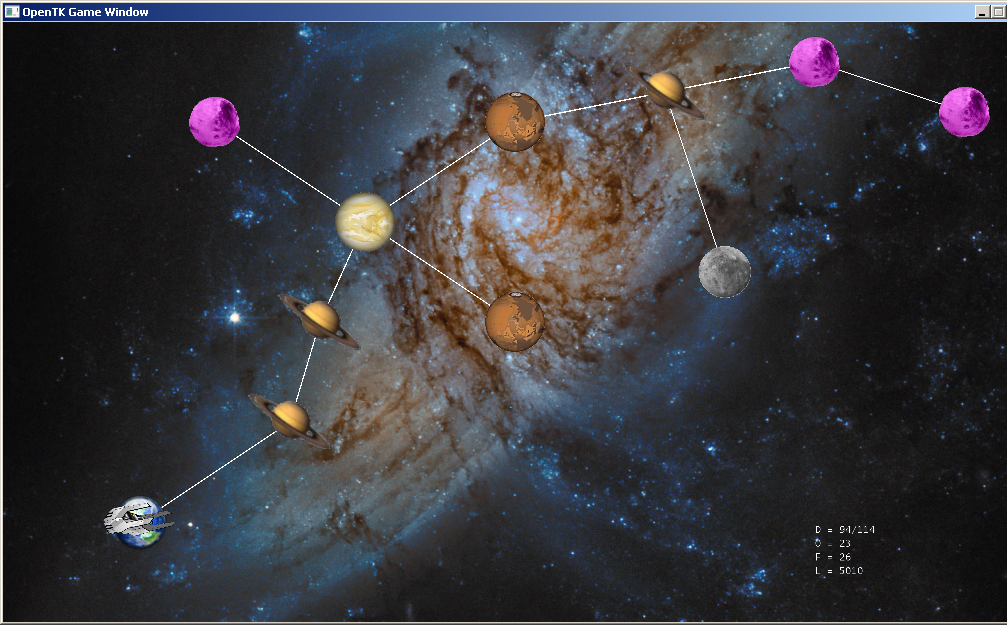
\includegraphics[width=4cm]{Pics/pic.png}
\caption{A planning AI simulator prototype}
\label{fig:AI-prototype}
\end{figure}
\end{block}
\end{frame}


\begin{frame}[fragile]{Graphs with tikz-qtree package}
\begin{lstlisting}
\Tree [.S [.NP [.Det poesje ] [.N mauw ] ] ]
\end{lstlisting}
\begin{block}{Result}
\Tree [.S [.NP [.Det poesje ] [.N mauw ] ] ]
\end{block}
\end{frame}


\begin{frame}[fragile]{Code}
\begin{verbatim}
\begin{lstlisting}[language=pascal]
for i:=maxint to 0 do
begin
{ do nothing }
end;
Write('Hello world ');
\end{lstlisting}
\end{verbatim}
\begin{block}{Result}
\begin{lstlisting}[language=pascal]
for i:=maxint to 0 do
begin
{ do nothing }
end;
Write('Hello world ');
\end{lstlisting}
\end{block}
\end{frame}


\begin{frame}[fragile]{Math - subscripts and superscripts}
\begin{lstlisting}
$x^2
x_i
x^2_{i+1}$
\end{lstlisting}
\begin{block}{Result}
$x^2
x_i
x^2_{i+1}$
\end{block}
\end{frame}


\begin{frame}[fragile]{Math - Greek letters}
\begin{lstlisting}
$\alpha^{\beta_\gamma} + \Omega = \aleph_0$
\end{lstlisting}
\begin{block}{Result}
$\alpha^{\beta_\gamma} + \Omega = \aleph_0$
\end{block}
\end{frame}


\begin{frame}[fragile]{Math - operators}
\begin{lstlisting}
$\top \bot \emptyset \exists \forall \neg \| 
\cdot \times \div \odot \oplus \dots$
\end{lstlisting}
\begin{block}{Result}
$\top\ \bot\ \emptyset\ \exists\ \forall\ \neg\ \|\ \cdot\ \times\ \div\ \odot\ \oplus$
\end{block}
\end{frame}


\begin{frame}[fragile]{Math - operators}
\begin{lstlisting}
$\leq \geq \equiv \sim \simeq \models \perp \parallel \ll \subset \in \vdash \ni \not< \not\leq \not= \not\simeq$
\end{lstlisting}
\begin{block}{Result}
$\leq\ \geq\ \equiv\ \sim\ \simeq\ \models\ \perp\ \parallel\ \ll\ \subset\ \in\ \vdash\ \ni\ \not<\ \not\leq\ \not=\ \not\simeq$
\end{block}
\end{frame}


\begin{frame}[fragile]{Math - arrows}
\begin{lstlisting}
$\leftarrow \rightarrow \Leftarrow \Longrightarrow \Longleftrightarrow \hookrightarrow$
\end{lstlisting}
\begin{block}{Result}
$\leftarrow\ \rightarrow\ \Leftarrow\ \Longrightarrow\ \Longleftrightarrow\ \hookrightarrow$
\end{block}
\end{frame}

\begin{frame}[fragile]{Math - fractional and root}
\begin{lstlisting}
$\frac{-b \pm \sqrt{b^2 - 4ac}}{2a}$
\end{lstlisting}
\begin{block}{Result}
$\frac{-b \pm \sqrt{b^2 - 4ac}}{2a}$
\end{block}
\end{frame}


\begin{frame}[fragile]{Math - non-square roots}
\begin{lstlisting}
$\sqrt[3]{q + \sqrt{ q^2 - p^3 }} + \sqrt[3]{q - \sqrt{ q^2 - p^3 }}$\end{lstlisting}
\begin{block}{Result}
$\sqrt[3]{q + \sqrt{ q^2 - p^3 }} + \sqrt[3]{q - \sqrt{ q^2 - p^3 }}$
\end{block}
\end{frame}


\begin{frame}[fragile]{Math - predefined functions}
\begin{lstlisting}
$\cos(\theta + \phi) = \cos \theta \cos \phi - \sin \theta \sin \phi$
\end{lstlisting}
\begin{block}{Result}
$\cos(\theta + \phi) = \cos \theta \cos \phi - \sin \theta \sin \phi$
\end{block}
\end{frame}

\begin{frame}[fragile]{Math - custom functions}
\begin{lstlisting}
$\operatorname{arg\,max}_a f(a) = \operatorname*{arg\,max}_b f(b)$
\end{lstlisting}
\begin{block}{Result}
$\operatorname{arg\,max}_a f(a) = \operatorname*{arg\,max}_b f(b)$
\end{block}
\end{frame}


\begin{frame}[fragile]{Math - custom functions declaration}
\begin{lstlisting}
\DeclareMathOperator*{\argmax}{arg\,max}

$\argmax_c f(c)$
\end{lstlisting}
\begin{block}{Result}
$\argmax_c f(c)$
\end{block}
\end{frame}


\begin{frame}[fragile]{Math - ellipsis}
\begin{lstlisting}
$f(x_1, x_2,\ldots, x_n) = x_1^2 + x_2^2 + \cdots + x_n^2$
\end{lstlisting}
\begin{block}{Result}
$f(x_1, x_2,\ldots, x_n) = x_1^2 + x_2^2 + \cdots + x_n^2$
\end{block}
\end{frame}


\begin{frame}[fragile]{Math - norm}
\begin{lstlisting}
$\|f\|$
\end{lstlisting}
\begin{block}{Result}
$\|f\|$
\end{block}
\end{frame}


\begin{frame}[fragile]{Math - brackets}
\begin{lstlisting}
$f(x,y,z) = 3y^2 z \left( 3 + \frac{7x+5}{1 + y^2} \right)$
\end{lstlisting}
\begin{block}{Result}
$f(x,y,z) = 3y^2 z \left( 3 + \frac{7x+5}{1 + y^2} \right)$
\end{block}
\end{frame}


\begin{frame}[fragile]{Math - brackets}
\begin{lstlisting}
$\left| 4 x^3 + \left( x + \frac{42}{1+x^4} \right) \right|$
\end{lstlisting}
\begin{block}{Result}
$\left| 4 x^3 + \left( x + \frac{42}{1+x^4} \right) \right|$
\end{block}
\end{frame}


\begin{frame}[fragile]{Math - empty brackets}
\begin{lstlisting}
$\left. \frac{du}{dx} \right|_{x=0}$
\end{lstlisting}
\begin{block}{Result}
$\left. \frac{du}{dx} \right|_{x=0}$
\end{block}
\end{frame}


\begin{frame}[fragile]{Math - multi-line equations}
\begin{lstlisting}
\begin{eqnarray*}
\cos 2\theta & = & \cos^2 \theta - \sin^2 \theta \\
             & = & 2 \cos^2 \theta - 1.
\end{eqnarray*}
\end{lstlisting}
\begin{block}{Result}
\begin{eqnarray*}
\cos 2\theta & = & \cos^2 \theta - \sin^2 \theta \\
             & = & 2 \cos^2 \theta - 1.
\end{eqnarray*}
\end{block}
\end{frame}


\begin{frame}[fragile]{Math - matrices}
\begin{lstlisting}
$\left( \begin{array}{ccc}
a & b & c \\
d & e & f \\
g & h & i \end{array} \right)$
\end{lstlisting}
\begin{block}{Result}
$\left( \begin{array}{ccc}
a & b & c \\
d & e & f \\
g & h & i \end{array} \right)$
\end{block}
\end{frame}


\begin{frame}[fragile]{Math - systems of equations}
\begin{lstlisting}
$ |x| = \left\{ \begin{array}{ll}
         x & \mbox{if $x \geq 0$};\\
        -x & \mbox{if $x < 0$}.\end{array} \right.$
\end{lstlisting}
\begin{block}{Result}
$ |x| = \left\{ \begin{array}{ll}
         x & \mbox{if $x \geq 0$};\\
        -x & \mbox{if $x < 0$}.\end{array} \right.$
\end{block}
\end{frame}


\begin{frame}[fragile]{Math - derivatives}
\begin{lstlisting}
$\frac{\partial u}{\partial t}$
\end{lstlisting}
\begin{block}{Result}
$\frac{\partial u}{\partial t}$
\end{block}
\end{frame}


\begin{frame}[fragile]{Math - limits}
\begin{lstlisting}
$\lim_{x \to +\infty} \frac{3x^2 +7x^3}{x^2 +5x^4} = 3$
\end{lstlisting}
\begin{block}{Result}
$\lim_{x \to +\infty} \frac{3x^2 +7x^3}{x^2 +5x^4} = 3$
\end{block}
\end{frame}


\begin{frame}[fragile]{Math - summations}
\begin{lstlisting}
$\sum_{k=1}^n k^2 = \frac{1}{2} n (n+1)$
\end{lstlisting}
\begin{block}{Result}
$\sum_{k=1}^n k^2 = \frac{1}{2} n (n+1)$
\end{block}
\end{frame}


\begin{frame}[fragile]{Math - integrals}
\begin{lstlisting}
$\int_a^b f(x)\,dx$
\end{lstlisting}
\begin{block}{Result}
$\int_a^b f(x)\,dx$
\end{block}
\end{frame}


\begin{frame}[fragile]{Bibliography}
\begin{lstlisting}
\bibliographystyle{plain}
\bibliography{bibliography}
\end{lstlisting}
\end{frame}


\begin{frame}[fragile]{Bibliography}
\begin{lstlisting}
@article{LAMBDA_CALCULUS,
    author = {Church, Alonzo},
    journal = {Annals of Mathematics},
    number = {33},
    pages = {346--366},
    posted-at = {2010-10-04 02:27:47},
    priority = {2},
    title = {{A Set of Postulates for the Foundation of Logic}},
    url = {http://www.jstor.org/stable/1968337},
    volume = {2},
    year = {1932}
}
\end{lstlisting}
\end{frame}


\begin{frame}[fragile]{References}
\begin{lstlisting}
As we see in \cite{LAMBDA_CALCULUS}, ...
\end{lstlisting}
\begin{block}{Result}
As we see in \cite{LAMBDA_CALCULUS}, ...
\end{block}
\end{frame}


\begin{frame}[allowframebreaks]{Bibliography}
\bibliographystyle{plain}
\bibliography{bibliography}
\end{frame}


\end{document}